\documentclass[hidelinks]{article}

\usepackage[english]{babel}
%% Verwende Umlaute direkt
\usepackage[utf8x]{inputenc}
%% Hyperlinks für interne Referenzen
\usepackage{hyperref}
\hypersetup{
    colorlinks,
    linkcolor={red!50!black},
    citecolor={blue!50!black},
    linktoc=all,
    urlcolor={blue!80!black}
}
%% Grafiken einbinden
\usepackage{graphicx}
\usepackage{float}
%% Paket für Unterabbildungen pro Abbildung
\usepackage{subfig}

\usepackage{forloop}

\usepackage{enumerate}
\usepackage{amsmath}
\usepackage{amssymb}
\usepackage{algorithm}
\usepackage[noend]{algpseudocode}
\newcommand\Let[2]{\State #1 $\gets$ #2}
\algrenewcomment[1]{\(\qquad \triangleright\) #1}
\newcommand\Blet[2]{\State \textbf{let} #1 \textbf{be} #2}

\usepackage{mathtools}
% Proof system
\usepackage{amsthm}

\theoremstyle{plain}
\newtheorem{thm}{Theorem}[section]
\newtheorem{lem}{Lemma}[section]
\newtheorem{prop}{Proposition}[section]

\theoremstyle{definition}
\newtheorem{defn}[thm]{Definition}
\newtheorem{bsp}[thm]{Example}

\newtheoremstyle{rem} % name
    {\topsep}                    % Space above
    {\topsep}                    % Space below
    {}                   % Body font
    {}                           % Indent amount
    {\bf}                   % Theorem head font
    {:}                          % Punctuation after theorem head
    {.5em}                       % Space after theorem head
    {}  % Theorem head spec (can be left empty, meaning ‘normal’)

\theoremstyle{rem}
\newtheorem*{remark}{Note}

%\usepackage{xpatch}
%\makeatletter
%% Remove last point from definitions, theorems, etc.
%\xpatchcmd{\@thm}{\thm@headpunct{.}}{\thm@headpunct{\\}}{}{}
%\makeatother

% Seitenränder
%TODO originally 1.5 in
\usepackage[margin=1.3in]{geometry}
% Zitate
\usepackage{cite}
% Tabellen
\usepackage[table]{xcolor}

% Graphs
\usepackage{tikz}
\usetikzlibrary{calc,arrows.meta,positioning}
\usepackage{tikz-3dplot}
\usepackage{pgfplots}

\setlength{\parindent}{0pt}

% Titel der Arbeit
\title{Power management - Dynamic Programming}
% Angaben zum Author
\author{Kevin Kappelmann\\
  \multicolumn{1}{p{.7\textwidth}}{\centering\emph{Chair for Theoretical Computer Science,\\
  Technical University of Munich}}}  

\pagestyle{plain}

%------------------------------------------------------------------------------
\begin{document}

\pagenumbering{arabic}

\begin{sloppypar}
\section{Optimal scheduling for m homogeneous servers}
TODO: introduction text
\subsection{Input and conventions}
TODO: rewrite in nice paragraph\\
Input:
\begin{itemize}
	\item $m$: Number of homogeneous servers
	\item $T$: Number of time steps
	\item $\beta$: Power up costs
	\item $\lambda_0,\ldots,\lambda_{T}\in[0,m]$: Arrival rates
\end{itemize}
Notations:
\begin{itemize}
	\item Let $\lambda_{i,t}$ be the assigned arrival rate at time t for server i
	\item Let $\mathcal{X}=(x_0,\ldots,x_T)$ be the number of active servers at time t
\end{itemize}
Requirements:
\begin{itemize}
	\item Convex cost function $f$
	\item Power down costs are w.l.o.g.\ equal to 0
	\item $\forall t\in \{0,\ldots,T\}:\sum\limits_{i=1}^{m}{\lambda_{i,t}=\lambda_t}$
	\item $\lambda_0=\lambda_T=0$
	\item $\mathcal{X}(0)=\mathcal{X}(T)=0$, i.e.\ all servers are powered down at $t=0$ and $t=T$
\end{itemize}

\subsection{Preliminaries}
We show that given a convex cost function $f$, for $x$ active servers and an arrival rate $\lambda$, the best method is to assign each server a load of $\lambda/x$:\\
$\forall x\in\mathbb{N},\mu_i\in[0,1]:\sum\limits_{i=1}^{x}{\mu_i}=1:$
\begin{alignat}{5}
	f\Bigl(\frac{\lambda}{x}\Bigr)=&&f\Bigl(\sum\limits_{i=1}^x{\frac{\mu_i*\lambda}{x}}\Bigr)&\stackrel{\text{Jensen's inequality}}{\le}&&\sum\limits_{i=1}^x\frac{1}{x}f(\mu_i*\lambda) \nonumber\\
	\Leftrightarrow&&x*f\Bigl(\frac{\lambda}{x}\Bigr)&\qquad\quad\le&&\sum\limits_{i=1}^xf(\mu_i*\lambda) \label{eq:balance}
\end{alignat}
We will use this fact in our following construction for an optimal schedule.

\subsection{Graph for an optimal schedule}
We construct a directed acyclic graph as follows:\\
$\forall t\in[T-1]$ and $i,j\in\{0,\ldots,m\}$ we add vertices $(t,i)$ modelling the number of active servers at time t. Furthermore, we add vertices $(0,0)$ and $(T,0)$ for our initial and final state respectively.\\
In order to warrant that there are at least $\lceil\lambda_t\rceil$ active servers $\forall t\in[T-1]$, we define an auxiliary function which calculates the costs for handling an arrival rate $\lambda$ with $x$ active servers:
\begin{equation}
	c(x,\lambda)\coloneqq\begin{cases}
	  x*f(\lambda/x), & \text{if $\lambda\le x$}\\
	  \infty, & \text{otherwise}
	  \end{cases} \label{fct:c}
\end{equation}
Then, $\forall t\in[T-2]$ and $i,j\in\{0,\ldots,m\}$ we add edges from $(t,i)$ to $(t+1,j)$ with weight
\begin{equation}
	d(i,j,\lambda_{t+1})\coloneqq\underbrace{\beta*\min\{0,j-i\}}_{\text{power up costs}}+c(j,\lambda_{t+1})
\end{equation}
Finally, for $0\le i\le m$ we add edges from $(0,0)$ to $(1,i)$ with weight $d(0,i,\lambda_1)$ and from $(T-1,i)$ to $(T,0)$ with weight $d(i,0,\lambda_T)=0$.
\begin{figure}[H]
\centering
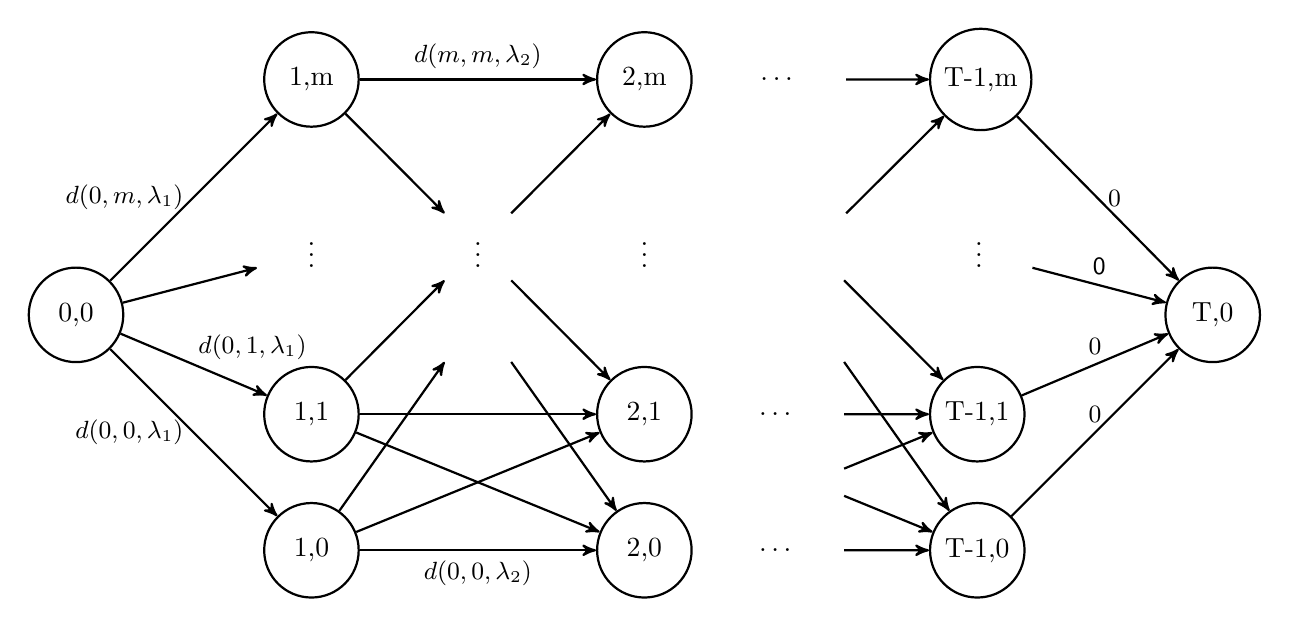
\begin{tikzpicture}[->,>=stealth',auto,node distance=3cm,thick,node/.style={minimum size=1.2cm,circle,draw}]

  \node[node] (1) {0,0};
  \node[node] (4) [below right =of 1] {1,0};
  \node[node] (3) [above =0.5cm of 4] {1,1};
  \node[node] (2) [above right=of 1] {1,m};
  \node[node] (6) [right =of 3] {2,1};
  \node[node] (5) [right =of 2] {2,m};
  \node[node] (7) [right =of 4] {2,0};
  \node[node] (9) [right =of 6] {T-1,1};
  \node[node] (8) [right =of 5] {T-1,m};
  \node[node] (10) [right =of 7] {T-1,0};
  \node[node] (11) [above right =of 10] {T,0};

  \node at ($(5)!.4!(8)$) {\ldots};
  \node at ($(6)!.4!(9)$) {\ldots};
  \node at ($(7)!.4!(10)$) {\ldots};

  \node at ($(2)!.5!(3)$) {\vdots};
  \node at ($(2)!.5!(6)$) {\vdots};
  \node at ($(5)!.5!(6)$) {\vdots};
  \node at ($(8)!.5!(9)$) {\vdots};

  \path[every node/.style={font=\sffamily\small}]
    (1) edge node[left] {$d(0,m,\lambda_1)$} (2)
	edge node[above right=-0.1cm] {$d(0,1,\lambda_1)$} (3)
	edge node[left] {$d(0,0,\lambda_1)$} (4)
    (2) edge node[above] {$d(m,m,\lambda_2)$} (5)
    (3) edge (6)
	edge (7)
    (4) edge (6)
	edge node[below] {$d(0,0,\lambda_2)$} (7)
    (8) edge node[right] {$0$} (11)
    (9) edge node[above] {$0$} (11)
    (10) edge node[above] {$0$} (11);

   \path [->,draw,thick] (1) to ($(1)!.2!(8)$);
   \path [->,draw,thick] (2) to ($(2)!.4!(6)$);
   \path [->,draw,thick] (4) to ($(4)!.4!(5)$);
   \path [->,draw,thick] (3) to ($(3)!.4!(5)$);

   \path [->,draw,thick] ($(3)!.6!(5)$) to (5);
   \path [->,draw,thick] ($(2)!.6!(6)$) to (6);
   \path [->,draw,thick] ($(2)!.6!(7)$) to (7);

   \path [->,draw,thick] ($(6)!.6!(8)$) to (8);
   \path [->,draw,thick] ($(5)!.6!(8)$) to (8);

   \path [->,draw,thick] ($(5)!.6!(9)$) to (9);
   \path [->,draw,thick] ($(6)!.6!(9)$) to (9);
   \path [->,draw,thick] ($(7)!.6!(9)$) to (9);

   \path [->,draw,thick] ($(5)!.6!(10)$) to (10);
   \path [->,draw,thick] ($(6)!.6!(10)$) to (10);
   \path [->,draw,thick] ($(7)!.6!(10)$) to (10);

   \path[every node/.style={font=\sffamily\small}] [->,draw,thick] ($(2)!.8!(11)$) -- node[above] {0} ++ (11);

\end{tikzpicture}
\caption{All edges from $(t,i)$ to $(t+1,j)$ have weight $d(i,j,\lambda_{t+1})$}
\end{figure}

\subsection{Proof of correctness}
\begin{prop}
Any given optimal schedule corresponds to a shortest path from $(0,0)$ to $(T,0)$ in the constructed graph and vice versa.
\end{prop} 
\begin{proof}
$ $
\begin{itemize}
	\item[``$\Rightarrow$'':] In equation~(\ref{eq:balance}) we have shown that in an optimal schedule each arrival rate $\lambda_t$ will be shared equally on each active server at time t. Therefore, we can denote an optimal schedule uniquely by the sequence $\mathcal{X}$ of active servers.\\
We can construct a valid path in our graph from $\mathcal{X}$ as follows:\\
$\forall t\in[T]$ set $e_t\coloneqq\Bigl(\bigl(t-1,\mathcal{X}(t-1)\bigr),\bigl(t,\mathcal{X}(t)\bigr)\Bigr)$. Then set $P\coloneqq(e_1,\ldots,e_{T})$.\\
As each edge $e_t$ in our graph has weight $d\bigl(\mathcal{X}(t-1),\mathcal{X}(t),\lambda_{t}\bigr)$ and hence corresponds to the costs of switching from $\mathcal{X}(t-1)$ to $\mathcal{X}(t)$ servers and processing $\lambda_{t}$ with $\mathcal{X}(t)$ active servers, it directly follows that $P$ is a shortest path of the graph.

	\item[``$\Leftarrow$'':] Let $P=\bigl((0,0)=v_0,\ldots,v_T=(T,0)\bigr)$ with $v_t\in\bigl\{(t,i)\mid 0\le i\le m\bigr\}$ be a shortest path of the graph. Again, it follows from equation~(\ref{eq:balance}) that an optimal schedule is uniquely identified by the sequence $\mathcal{X}$ of active servers.\\
We can construct a schedule from $P$ by setting $\mathcal{X}=\bigl(v_0(1),\ldots,v_T(1)\bigr)$ where $v_t(1)$ is the second component of the t-th tuple in $P$.\\
By definition~(\ref{fct:c}) it is guaranteed that $P$ only traverses edges such that there are enough active servers $\forall t\in[T]$. Therefore, the created schedule is feasible. It's optimality directly follows from the definition of the edges' weights.\\
\end{itemize}
\end{proof}

\subsection{A minimum cost algorithm}
\begin{algorithm}[H]
    \caption{Calculate costs for $m$ homogeneous servers}
    \begin{algorithmic}[1]
        \Require{Convex cost function $f$, $\lambda_0=\lambda_T=0$, $\forall t\in[T-1]:\lambda_t\in[0,m]$}
   \Function{schedule}{$m,T,\beta,\lambda_1,\ldots,\lambda_{T-1}$}
	\If{$T<2$} \Return
	\EndIf
	\Blet{$p[2\ldots T-1,m]$ and $M[1\ldots T-1,m]$}{new arrays}
	\For{$j \gets 0 \textrm{ to } m$}
		\Let{$M[1,j]$}{$d(0,j,\lambda_1)$}
	\EndFor
	\For{$t \gets 1 \textrm{ to } T-2$}
		\For{$j \gets 0 \textrm{ to } m$}
			\Let{$opt$}{$\infty$}
			\For{$i \gets 0 \textrm{ to } m$}
				\Let{$M[t+1,j]$}{$M[t,i]+d(i,j,\lambda_{t+1})$}
				\If{$M[t+1,j]<opt$}
					\Let{$opt$}{$M[t+1,j]$}
					\Let{$p[t+1,j]$}{$i$}
				\EndIf
			\EndFor
			\Let{$M[t+1,j]$}{$opt$}
		\EndFor
	\EndFor
	\State \Return{$p$ and $M$}
  \EndFunction
  \end{algorithmic}
\end{algorithm}
\begin{algorithm}[H]
    \caption{Extract schedule for n homogeneous servers}
    \begin{algorithmic}[1]
   \Function{Extract}{$m,p,M,T$}
	\Blet{$x[0\ldots T]$}{a new array}
	\Let{$x[0]$}{$x[T]\leftarrow 0$}
	\If{$T<2$} \Return $x$ \Comment{Trivial solution}
	\EndIf
	\Let{$x[T-1]$}{$\underset{0\le i\le m}{arg\ min}\{M[T-1,i]\}$}
	\For{$t \gets T-2 \textrm{ to } 1$}
		\Let{$x[t]$}{$p[t+1,x[t+1]]$}
	\EndFor
	\State \Return{$x$}
  \EndFunction
  \end{algorithmic}
\end{algorithm}

\subsubsection{Runtime analysis}
Schedule: Loop 5,8 and 10 run $m+1$ times, loop 7 runs $T-2$ times\\
Extract: Loop 5 runs $T-2$ times, argmin 4 takes time $m+1$.\\
For $T,n\rightarrow\infty$ it holds:
\begin{equation}
	\mathcal{O}(m+1+(T-2)*(m+1)^2+T-2+m+1)=\mathcal{O}(2*m+T+(T-2)*(m+1)^2)=\mathcal{O}(T*m^2) 
\end{equation}
As we need $\log_2(m)$ bits to encode m, the algorithm is exponential in the number of servers.

\end{sloppypar}
\end{document}
